\subsection{参数、精度与证据范围}
新计算统一采用 $a=0.5$、固定入射归一化。粗细两档分别使用 320/384 bit，
内区阶数 64/80、外区阶数 48/64，积分阶数和 Levin 阶数独立提高。
当前共有 21 个配对参数点，其中 21 个通过预设接受门槛。
表中数字展示物理尺度；完整有效数字及逐项误差保存在 CSV 和 TOML 中。
\begin{longtable}{rrrrrr}
\caption{新标量非线性散射结果。$m=0$；$\mathcal S=|\chi|/[2\psi\sqrt{R^{(0)}/(1-R^{(0)})}]$。}\\
\toprule $\ell$ & $n$ & $\omega$ & $\chi_n$ & $\psi_n$ & $\mathcal S$\\\midrule\endfirsthead
\toprule $\ell$ & $n$ & $\omega$ & $\chi_n$ & $\psi_n$ & $\mathcal S$\\\midrule\endhead
0 & 1 & $1.0\times10^{-5}$ & $0.2206456$ & $0.2500066$ & $1.71\times10^{-5}$\\
0 & 2 & $1.0\times10^{-5}$ & $6.317813\times10^{-12}$ & $3.979159\times10^{-12}$ & $3.07\times10^{-5}$\\
0 & 3 & $1.0\times10^{-5}$ & $1.72461\times10^{-22}$ & $8.444427\times10^{-23}$ & $3.95\times10^{-5}$\\
1 & 1 & $1.0\times10^{-5}$ & $0.1471387$ & $0.2100021$ & $3.91\times10^{-11}$\\
2 & 1 & $1.0\times10^{-5}$ & $0.1063674$ & $0.1683684$ & $4.07\times10^{-17}$\\
0 & 1 & $1.0\times10^{-4}$ & $0.2207357$ & $0.2500659$ & $1.71\times10^{-4}$\\
1 & 1 & $1.0\times10^{-4}$ & $0.1471567$ & $0.2100212$ & $3.91\times10^{-9}$\\
2 & 1 & $1.0\times10^{-4}$ & $0.1063751$ & $0.1683779$ & $4.07\times10^{-14}$\\
0 & 1 & $1.0$ & $1.112854\times10^{-11}$ & $0.02087919$ & $3.56\times10^{-5}$\\
0 & 1 & $2.0$ & $6.401732\times10^{-23}$ & $0.01045553$ & $1.4\times10^{-10}$\\
0 & 1 & $3.0$ & $5.497823\times10^{-34}$ & $0.007311307$ & $5.26\times10^{-16}$\\
0 & 2 & $3.0$ & $1.551077\times10^{-35}$ & $5.889127\times10^{-5}$ & $1.84\times10^{-15}$\\
0 & 3 & $3.0$ & $-1.969823\times10^{-36}$ & $9.020307\times10^{-7}$ & $1.53\times10^{-14}$\\
1 & 1 & $3.0$ & $3.733594\times10^{-33}$ & $0.01392532$ & $9.53\times10^{-16}$\\
2 & 1 & $3.0$ & $8.793907\times10^{-32}$ & $0.01405412$ & $4.24\times10^{-15}$\\
0 & 1 & $5.0$ & $6.450157\times10^{-56}$ & $0.006337859$ & $6.56\times10^{-27}$\\
0 & 2 & $5.0$ & $2.326749\times10^{-57}$ & $9.093391\times10^{-5}$ & $1.65\times10^{-26}$\\
0 & 3 & $5.0$ & $-1.578132\times10^{-57}$ & $2.685534\times10^{-6}$ & $3.79\times10^{-25}$\\
0 & 1 & $10.0$ & $5.493329\times10^{-111}$ & $0.009108419$ & $1.75\times10^{-54}$\\
0 & 2 & $10.0$ & $9.421642\times10^{-113}$ & $3.836582\times10^{-4}$ & $7.13\times10^{-55}$\\
0 & 3 & $10.0$ & $-2.429499\times10^{-111}$ & $3.257994\times10^{-5}$ & $2.17\times10^{-52}$\\
\bottomrule\end{longtable}
\subsection{数值质量}
最大配对能流响应变化为 $1.362964\times10^{-19}$，
最大配对相位变化为 $1.478465\times10^{-40}$。
最高采样径向残差为 $4.514484\times10^{-62}$。
最大谱尾指标为 $5.211527\times10^{-61}$，
五点匹配半径下的最大反射振幅相对展宽为 $3.896329\times10^{-47}$。
成功配对运行记录中的最大进程峰值内存约为 1314 MB。
该组精度陈述对应独立加密的一致性和离节点原方程检查；外部高精度标量参考列为待完成检验。
\begin{figure}[htbp]\centering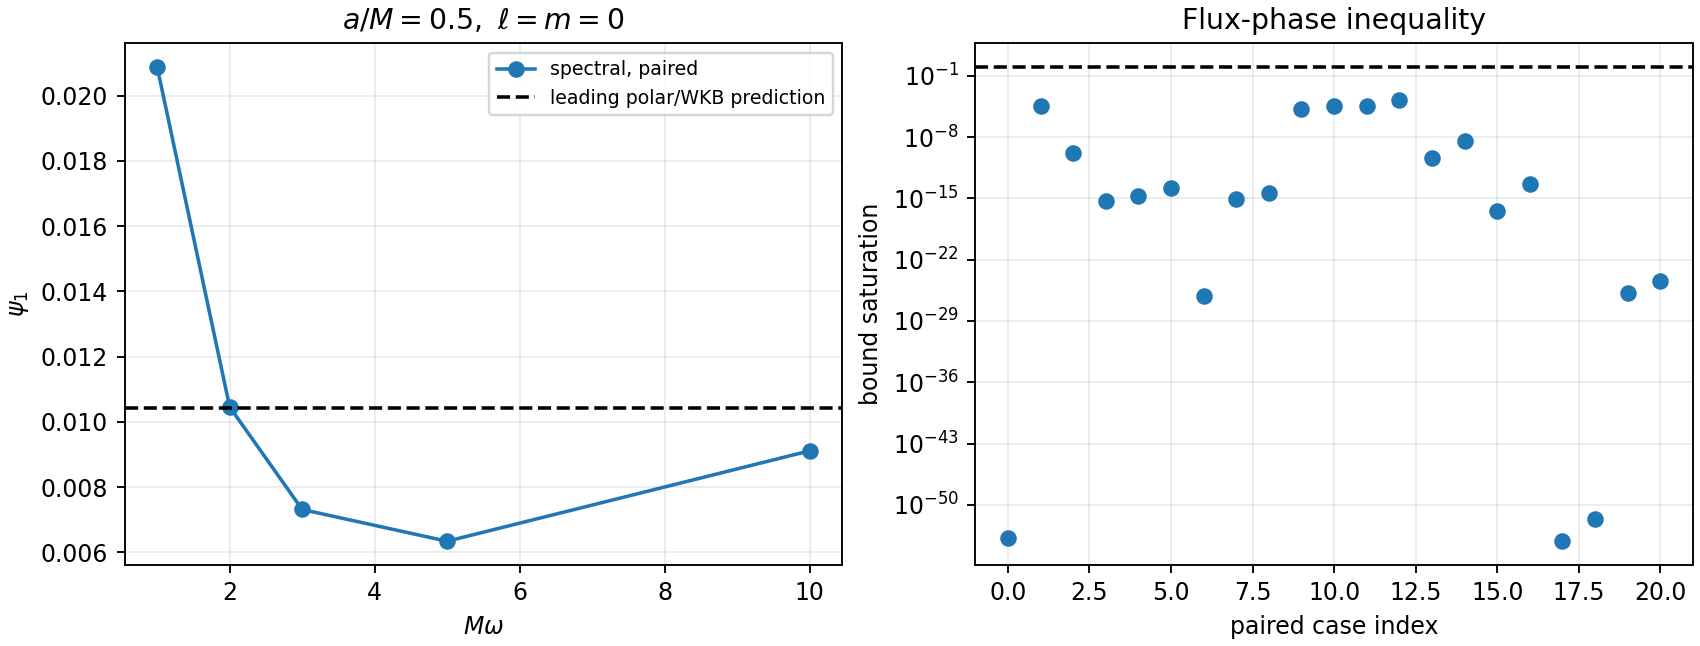
\includegraphics[width=.98\textwidth]{../../results/precision_20261023/response_summary.png}
\caption{新高精度标量结果。左：单极子三次响应的相位系数；右：各已配对点的不等式饱和比。}\end{figure}
